
\documentclass{beamer}
\usepackage{graphicx}
\usepackage{amsmath,amssymb,amstext,amsthm,xargs}
\usepackage{amsfonts}
\usepackage{bbm}
\usepackage{beamerthemesplit}

\usepackage[utf8]{inputenc}
\usepackage[french]{babel}
\usepackage{bbm}

\usetheme{Antibes}
\mode<presentation>
\useoutertheme{tree}
\usecolortheme{beaver}
\useinnertheme{rectangles}

\setbeamerfont{block title}{size={}}
%\usecolortheme[rgb={0.55,0.1,0.05}]{structure}
%\usecolortheme[rgb={0.75,0.1,0.05}]{structure}
\usepackage{color}

\newenvironment{disarray}{\everymath{\displaystyle\everymath{}}\array} {\endarray}
\newtheorem{theo}{Théorème}
\newtheorem{prop}[theo]{Proposition}
\newtheorem{conj}[theo]{Conjecture}
\newtheorem{cor}{Corollary}[theo]

\newtheorem{lem}{Lemme}
\newtheorem{nota}{Notation}
\newtheorem{rk}{Remark}
\newtheorem{exa}{Example}
\newtheorem{df}{Definition}
\newtheorem{terminologie}{Terminologie}
\def\rme{\mathrm{e}}
\def\rmi{\mathrm{i}}
\def\rset{\mathbb{R}}
\def\nset{\mathbb{N}}
\def\dlim{\stackrel{d}{\rightarrow}}
\newcommandx{\plim}[1][1=]{\stackrel{\PP_{#1}}{\longrightarrow}}
\def\iid{i.i.d.}
\def\1{\mathbbm{1}}
\newenvironment{dem}{\textbf{Proof}}{\flushright$\blacksquare$\\}
%\def\blankframe{
%\mode<presentation>{
%  { \setbeamertemplate{background canvas}[default]
%    \setbeamercolor{background canvas}{bg=black}
%    \begin{frame}[plain]{}
%    \end{frame}
%  }
%}
%\mode<presentation>{
%\setbeamertemplate{background canvas}[default]
%\setbeamercolor{background canvas}{bg=white}}
%\mode*
%}
\def\eqsp{\,}
\DeclareMathOperator{\E}{{\mathbb E}}
\def\PE{\E}
\def\PCov{\mathrm{Cov}}
\DeclareMathOperator{\F}{{\mathbb F}}
\DeclareMathOperator{\G}{{\mathbb G}}
\DeclareMathOperator{\D}{{\mathbb D}}
\DeclareMathOperator{\R}{{\mathbb R}}
\DeclareMathOperator{\C}{{\mathbb C}}
\DeclareMathOperator{\Z}{{\mathbb Z}}
\DeclareMathOperator{\N}{{\mathbb N}}
\DeclareMathOperator{\K}{{\mathbb K}}
\DeclareMathOperator{\T}{{\mathbb T}}
\DeclareMathOperator{\PP}{{\mathbb P}}
\DeclareMathOperator{\QQ}{{\mathbb Q}}
\DeclareMathOperator{\Q}{{\mathbb Q}}
\DeclareMathOperator{\IF}{{\mathbb I}}


%%%%%%%%%%%%%%%%%%%%%%%%%%%%%%% Pour le modèle lin\'eaire

\DeclareMathOperator{\bX}{\boldsymbol{X}}
\DeclareMathOperator{\bY}{\boldsymbol{Y}}
\DeclareMathOperator{\bx}{\boldsymbol{x}}
\DeclareMathOperator{\vp}{\boldsymbol{p}}
\DeclareMathOperator{\vq}{\boldsymbol{q}}
\DeclareMathOperator{\estMCNL}{\widehat \theta_n^{\,\,{\tt mcnl}}}
\DeclareMathOperator{\estMV}{\widehat \theta_n^{\,\,{\tt mv}}}
\DeclareMathOperator{\est}{\widehat \theta_{\mathnormal{n}}}
\DeclareMathOperator{\var}{\mathrm{Var}}
\def\Var{\var}
\DeclareMathOperator{\estMVc}{\widehat \theta_{n,0}^{\,{\tt mv}}}
\DeclareMathOperator{\Xbar}{\overline{\mathnormal{X}}_\mathnormal{n}}

\newcommand{\indi}[1]{\mathbbm{1}_{\{#1\}}}
\newcommand{\coint}[1]{\left[#1\right)}
\newcommand{\ocint}[1]{\left(#1\right]}
\newcommand{\ooint}[1]{\left(#1\right)}
\newcommand{\ccint}[1]{\left[#1\right]}

\definecolor{LightYell}{rgb}{0.95,0.83,0.70}
\definecolor{orange}{rgb}{1.0,0.50,0.01}
\definecolor{StroYell}{rgb}{0.95,0.88,0.72}
\definecolor{lightred}{rgb}{0.75,0.033,0}
\definecolor{shadecolor1}{rgb}{0.90,0.83,0.70}
\definecolor{myem}{rgb}{0.797,0.598,0.598}
\definecolor{BrickRed}{cmyk}{0,0.89,0.94,0.28}
\definecolor{RoyalPurple}{cmyk}{0.75,0.9,0,0}

\newcommand{\tco}[1]{\textcolor{orange}{#1}}
\newcommand{\tcr}[1]{\textcolor{lightred}{#1}}

\def\gauss{\mathcal{N}}
\def\truetheta{\theta}
\def\truebeta{\boldsymbol{\beta}}
\def\projX{A}
\def\curtheta{\alpha}
\def\argmin{\mathrm{argmin}}
\def\ie{\emph{i.e.}}
\def\regressmat{\mathbb{X}}
\def\errpred{\boldsymbol{\hat{\xi}}}
\def\bnoise{\boldsymbol{\xi}}
\def\predY{\hat{\mathbf{Y}}}
\DeclareMathOperator{\estregress}{\widehat{\truebeta}_n}
\DeclareMathOperator{\estMC}{\widehat \theta_n^{\,\,{\tt mc}}}
\def\curbeta{b}
\def\bcurbeta{\mathbf{b}}
\newcommand{\indep}{\rotatebox[origin=c]{90}{$\models$}} 
\newcommand{\Id}[1]{\mathrm{Id}_{#1}}

\title{MAP 433 : Introduction aux méthodes statistiques. Cours 5}
%\author{M. Hoffmann}
%\institute{Université Paris-Est and ETG}
\begin{document}
\date{25 Septembre 2015}
\maketitle



\begin{frame}
\frametitle{Aujourd'hui}
\tableofcontents
\end{frame}


\section{Méthode d'estimation dans le modèle de régression}

\subsection{Modèle de régression}

\begin{frame}
\frametitle{Influence d'une variable sur une autre}
\begin{itemize}
\item \underline{Principe} : on part de \alert{l'observation} d'un $n$-échantillon
$$Y_1,\ldots, Y_n\;\;\;(Y_i \in \R)$$
\item A chaque observation $Y_i$ est associée une \alert{observation auxiliaire} $\bX_i \alert{ \in \R^k}$.
\item On \alert{suspecte} l'échantillon
$$\bX_1,\ldots, \bX_n\;\;\;\alert{ (\bX_i \in \R^k)}$$
de contenir la \og majeure partie de la variabilité des $Y_i$ \fg{}.
\end{itemize}
\end{frame}

\begin{frame}
\frametitle{Modélisation de l'influence}
\begin{itemize}
\item Si $\bX_i$ contient \alert{toute la variabilité} de $Y_i$, alors $Y_i$ est mesurable par rapport à $\bX_i$ : il existe $r:\R^k\rightarrow \R$ telle que
$$Y_i = r\big(\bX_i\big),$$
mais peu réaliste (ou alors \alert{problème d'interpolation
numérique}).
\item \underline{Alternative} : représentation précédente avec \alert{ erreur additive} : on \alert{ postule}
$$Y_i = r\big(\bX_i\big)+\xi_i,$$
$\xi_i$ erreur aléatoire centrée (pour des raisons d'identifiabilité).
\end{itemize}
\end{frame}

\begin{frame}
\frametitle{Motivation: meilleure approximation $L^2$}
\begin{itemize}
\item \underline{Meilleure approximation $L^2$}. Si
$\E\big[Y^2\big]<+\infty$, la meilleure approximation de $Y$ par une
variable aléatoire $\bX$-mesurable est donnée par
\alert{l'espérance conditionnelle} $\E\big[Y|\bX\big]$ :
$$\E\big[\big(Y-r(\bX)\big)^2\big] = \min_h \E\big[\big(Y-h(\bX)\big)^2\big]$$
\item o\`u
$$r(\bx) = \E\big[Y|\bX=\bx\big],\;\;\bx \in \R^k.$$
\item On appelle $r(\cdot)$ \alert{fonction de régression de $Y$ sur
$\bX$}.
\end{itemize}
\end{frame}

\begin{frame}
\frametitle{Régression}
\begin{itemize}
\item On définit:
$$\xi = Y-\E\big[Y|\bX \big]\;\;\Longrightarrow\; \E\big[\xi\big]=0.$$
\item On a alors naturellement la représentation désirée
$$Y=r(\bX)+\xi, \quad \E\big[\xi\big]=0$$
si l'on pose
$$\boxed{r(\bx) = \E\big[Y|\bX=\bx\big],\;\;\bx \in \R^k}$$

\item On observe alors un $n$-échantillon
$$(\bX_1,Y_1),\ldots, (\bX_n,Y_n)$$
où
$$Y_i = r(\bX_i)+\xi_i,\;\;\E\big[\xi_i\big]=0$$
avec comme \alert{paramètre la fonction $r(\cdot)$}+ un \alert{jeu d'hypothèses} sur la loi des $\xi_i$.
\end{itemize}
\end{frame}

\begin{frame}
\frametitle{régresseurs aléatoires}
\begin{df}
Modèle de régression \alert{à design aléatoire} = donnée de
l'observation
$$(\bX_1,Y_1),\ldots, (\bX_n,Y_n)$$
avec $(Y_i,\bX_i)\in \R\times \R^k$ \alert{i.i.d.},
et\\\vspace{3mm} \centerline{$Y_i =
r(\alert{\truebeta},\bX_i)+ \sigma \xi_i,\;\;
\E\big[\xi_i|\bX_i\big]=0,\;\;\alert{
\truetheta \in \Theta \subset \R^d}.$}
\begin{itemize}
\item $\bx \leadsto r(\alert{\truebeta},\bx)$ fonction de \alert{ régression}, connue au paramètre
$\truebeta$ près.
\item $\bX_i$ = variables explicatives, co-variables, prédicteurs;
$(\bX_1,\ldots,\bX_n)$ = \alert{design}.
\end{itemize}
\end{df}
\end{frame}


\subsection{Régression à design déterministe}


%\begin{frame}
%\frametitle{Modèle alternatif : signal+bruit}
%\begin{itemize}
%\item \underline{Principe} : \alert{sur un exemple}. On observe
%$$Y_i = r(\truetheta, i/n)+\xi_i,\;\;i=1,\ldots,n$$
%où $r(\alert{\truetheta},\cdot):[0,1]\rightarrow \R$ est une
%fonction connue au paramètre $\alert{\truetheta \in \Theta
%\subset \R^d}$ près, et les $\xi_i$ sont i.i.d.,
%$\E\big[\xi_i\big]=0$.
%\item \alert{ But} : reconstruire $r(\alert{\truetheta},\cdot)$ c'est-à-dire \alert{ estimer $\truetheta$}.
%\item Plus généralement, on observe
%$$Y_i = r(\truetheta, \bx_i)+\xi_i,\;i=1,\ldots, n$$
%où $\bx_1,\ldots, \bx_n$ sont des points de $\R^k$ \alert{
%déterministes}.
%\end{itemize}
%\end{frame}

\begin{frame}
\frametitle{Modèle de régression à design déterministe}
\begin{df}
Modèle de régression \alert{à design déterministe} = donnée de
l'observation
$$(\bx_1,Y_1),\ldots, (\bx_n,Y_n)$$
avec $Y_i \in \R, \bx_i\in \R^k$, et \\\vspace{3mm} \centerline{$Y_i
=
r(\alert{\truebeta},\bx_i)+ \sigma \xi_i,\;\;\E_{\truetheta}\big[\xi_i\big]=0,\;\;\alert{
\truetheta \in \Theta \subset \R^d \times \R_+}.$}
\begin{itemize}
%\item $\bx \leadsto r(\alert{\truetheta},\bx)$ fonction de \alert{ régression}, connue au paramètre
%$\truetheta$ près.
\item $\bx_i$ déterministes, donnés (ou choisis) : plan d'expérience, points du \og design\fg{}.
\item Hypothèses sur les $\xi_i$ : à débattre. \alert{Pour simplifier}, les variables $\xi_i$ sont centrées, $\PE_{\truetheta}[\xi_i]=0$,
décorrélées, $\PE_{\truetheta}[\xi_i \xi_j]= 0$ si $i \ne j$ et de variance unité $\PE[\xi_i^2]= 1$ \alert{ (homoscédasticité)}.
\item \alert{ Attention !} Les $Y_i$ ne sont \alert{pas identiquement distribuées}.
\end{itemize}
\end{df}

 \underline{Question}: Comment estimer $\truetheta=(\truebeta,\sigma)$ dans ce modèle?

\end{frame}

\begin{frame}
\frametitle{Régression gaussienne}


\begin{itemize}
\item  Modèle de régression à design déterministe :
$$Y_i =
r({\truebeta},\bx_i)+\ \sigma xi_i,\;\;\truetheta \in \Theta\subset  \R^d \times \rset_+.$$
\item  Supposons: $\xi_i \sim {\mathcal N}(0,1)$, i.i.d.
\item On a alors le modèle de \alert{régression gaussienne}.
Comment estimer $\truetheta$?  \alert{On sait expliciter la loi
de l'observation} $Z=(Y_1,\dots,Y_n)$ $\Longrightarrow$ appliquer le
principe du maximum de vraisemblance.

\item La loi de $Y_i$:
\begin{align*}
\PP^{Y_i}(dy) & = \frac{1}{\sqrt{2\pi \sigma^2}}\exp\big
(-\frac{1}{2\sigma^2}(y-r({\truebeta},\bx_i))^2\big)dy \\
& \ll dy.
\end{align*}

%d'où
%$$\PP^{(Y_1,\ldots, Y_n)}(dy_1\ldots dy_n) = \Big(\prod_{i=1}^n \frac{1}{\sqrt{2\pi \sigma^2}}\exp\big(-\frac{1}{2\sigma^2}(y-\truetheta^T\bx_i)\big)\Big) dy_1\ldots dy_n$$
\end{itemize}
\end{frame}

\begin{frame}
\frametitle{EMV pour régression gaussienne}
\begin{itemize}
\item  Le modèle $\{\PP_\truetheta^n \alert{ = \text{loi de }\;(Y_1,\ldots, Y_n)},\truetheta \in \R^k\}$ est \alert{dominé} par
$\mu^n(dy_1\ldots dy_n) = dy_1\ldots dy_n.$
\item D'où
\begin{align*}
 \frac{d\PP_\truetheta^n}{d\mu^n}(y_1,\ldots, y_n)
  =\; &\prod_{i=1}^n \tfrac{1}{\sqrt{2\pi \sigma^2}}\exp
  \big(-\tfrac{1}{2\sigma^2}(y_i-r({\truebeta},\bx_i))^2\big) \\
\;= & \tfrac{1}{(\sqrt{2\pi \sigma^2})^{n}}
\exp\big(-\tfrac{1}{2\sigma^2}\sum_{i =
1}^n\big(y_i-r({\truebeta},\bx_i)\big)^2\big).
\end{align*}
\item La fonction de vraisemblance
$$\boxed{{\mathcal L}_n(\truetheta, Y_1,\ldots, Y_n)
\propto \exp\Big(-\frac{1}{2\sigma^2}\sum_{i = 1}^n\big(Y_i-
r({\truebeta},\bx_i)\big)^2\Big)}$$
\end{itemize}
\end{frame}

\begin{frame}
\frametitle{Estimateur des moindres carrés} Maximiser la
\alert{ vraisemblance} en régression gaussienne = minimiser
la somme des carrés: $$ \sum_{i = 1}^ne
\big(Y_i-r({\truebeta},\bx_i)\big)^2 \to \min_{\truetheta \in\Theta}.
$$
\begin{df}
Estimateur des \alert{moindres carrés} : tout estimateur
$\estregress$ t.q. \centerline{$\estregress \in \arg \min_{\truebeta \in
\Theta}\sum_{i = 1}^n \big(Y_i-r({\truebeta},\bx_i)\big)^2.$}
\end{df}
\begin{itemize}
\item  L'EMC est un M-estimateur. Pour le
modèle de régression gaussienne: $\boxed{\rm EMV = EMC}$.
\item \alert{ Existence, unicité.}
\end{itemize}
\end{frame}

\subsection{La droite des moindres carrés}

\begin{frame}
\frametitle{Droite de régression}
\begin{itemize}
\item \underline{Modèle le plus simple}
$\boxed{r(\truebeta,x)= \truebeta_0 + \truebeta_1 x}$
$$\boxed{Y_i = \truebeta_0 + \truebeta_1 x_i+\xi_i,\;\;i=1,\ldots,n}$$
avec $\alert{\truebeta = (\truebeta_0,\truebeta_1)^T \in \R^2}$ et les
$(x_1,\ldots, x_n)$ données.
%\item Erreurs centrées: $\E\big[\xi_i\big]=0$, de variances $\E\big[\xi_i^2\big]$ finies.
\item L'estimateur des moindres carrés:
$$\alert{\estregress}=(\hat{\truebeta}_0, \hat{\truebeta}_1) =
\arg \min_{(\curbeta_0,\curbeta_1)\in \R^2}\sum_{i = 1}^n \big(Y_i- \curbeta_0 - \curbeta_1 x_i\big)^2.
$$
\item \alert{Solution explicite}
\end{itemize}
\end{frame}

\begin{frame}
\frametitle{Droite de régression}
\begin{itemize}
\item  Le minimum est caractérisé par les équations
\[
\begin{cases}
\curbeta_0 + \curbeta_1 n^{-1} \sum_{i=1}^n x_i &= n^{-1} \sum_{i=1}^n Y_i \\
\curbeta_0 n^{-1} \sum_{i=1}^n x_i + \curbeta_1 n^{-1} \sum_{i=1}^n x_i^2 &= n^{-1} \sum_{i=1}^n x_i Y_i \eqsp.
\end{cases}
\]
\item Notons $\bar{x}_n = n^{-1} \sum_{i=1}^n x_i$. Si le déterminant $\Delta_n \ne 0$ où
\[
\Delta_n = \left|
                 \begin{array}{cc}
                   1 & n^{-1} \sum_{i=1}^n x_i \\
                   n^{-1} \sum_{i=1}^n x_i &  n^{-1} \sum_{i=}^n x_i^2 \\
                 \end{array}
\right| = S_{xx} = n^{-1} \sum_{i=1}^n (x_i^2 - \bar{x}_n)^2 \eqsp,  \quad  \eqsp,
\]
alors ce système d'équations a une solution unique:
\[
\begin{cases}
\estregress_0 &= \bar{Y}_n - \estregress_1 \bar{x}_n  \\
\estregress_1 &= \frac{S_{xY}}{S_{xx}} \eqsp, \quad S_{xY}= n^{-1} \sum_{i=1}^n (x_i - \bar{X}_n) (Y_i - \bar{x}_n) \eqsp.
\end{cases}
\]
\end{itemize}
\end{frame}

\begin{frame}
\frametitle{Régression linéaire simple}
\begin{figure}[h]
\begin{center}
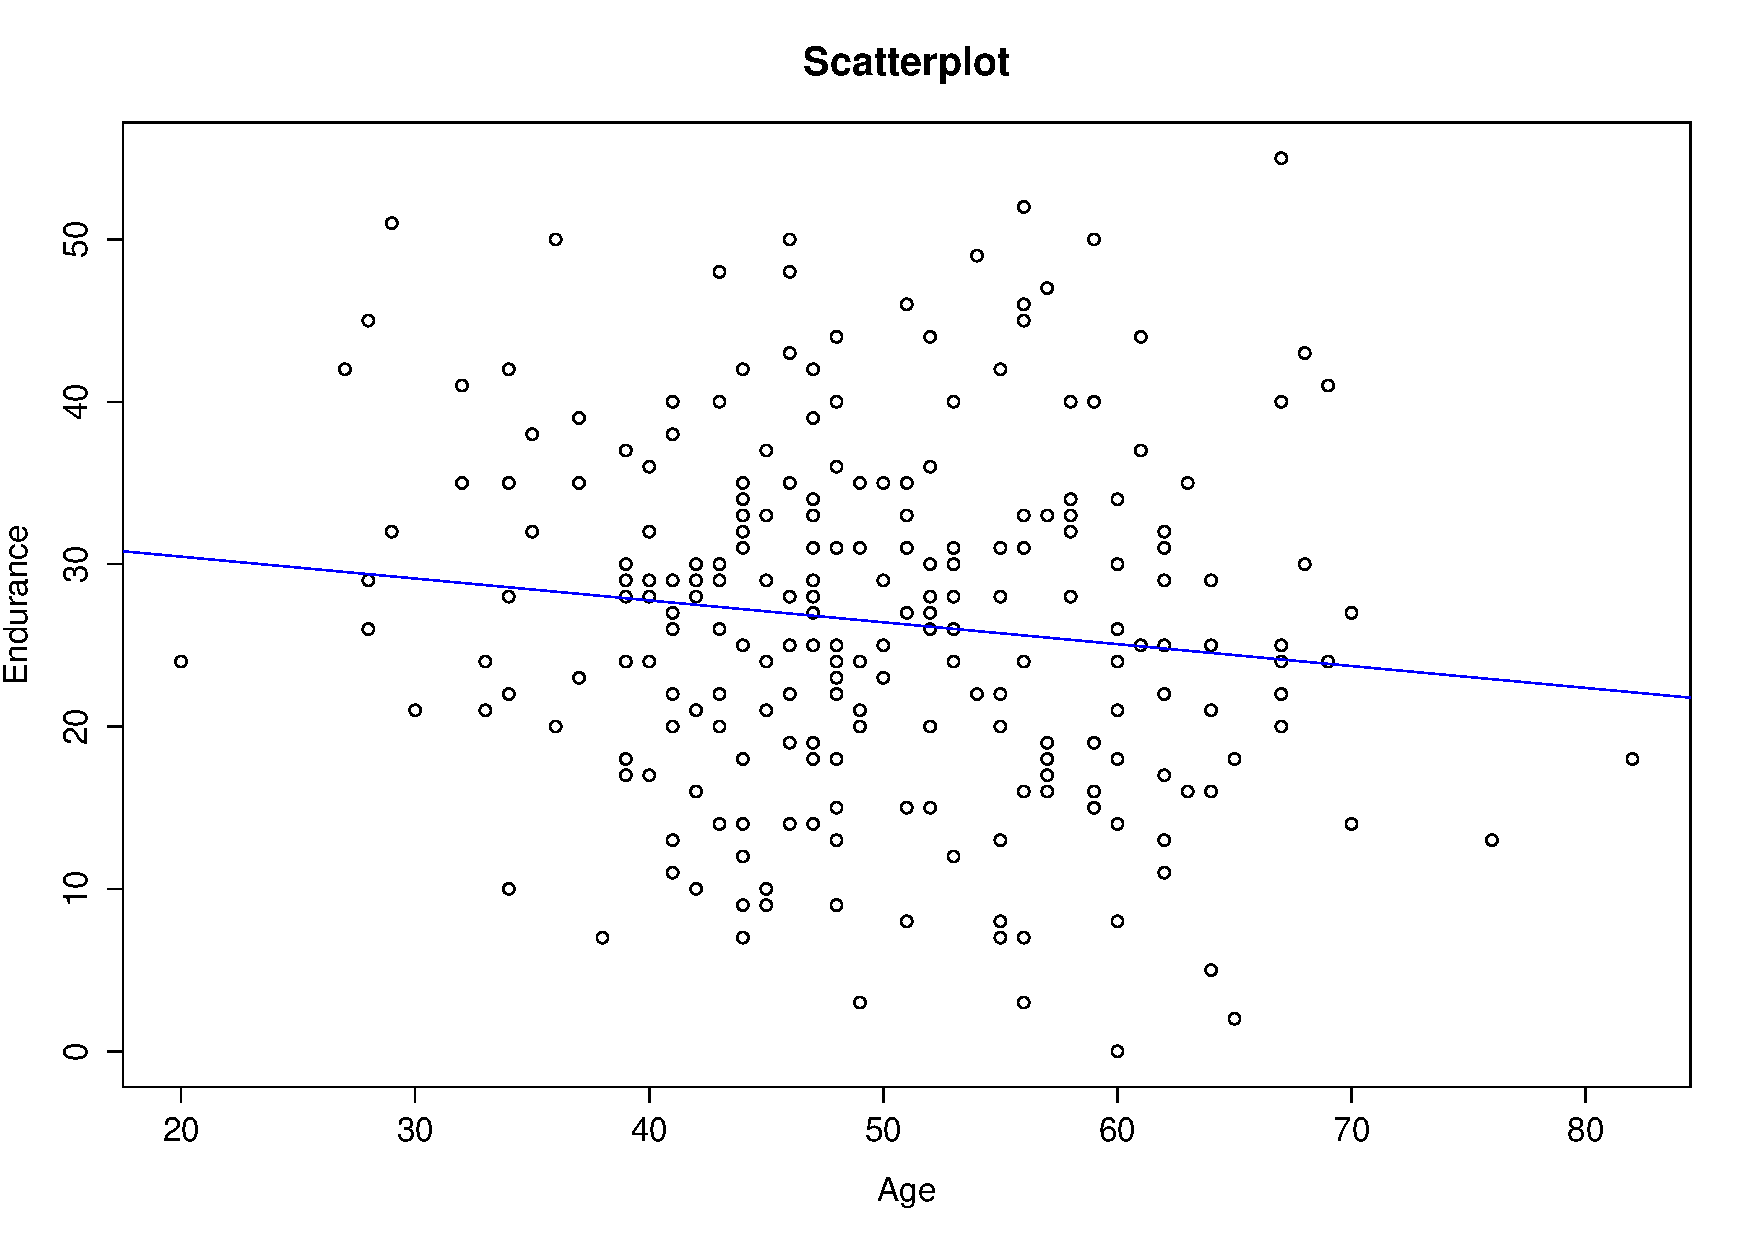
\includegraphics[width=0.9\textheight]{ScatterPlotEnduranceAge}
\end{center}
\end{figure}
\end{frame}

\begin{frame}
\frametitle{Régression linéaire simple}
\begin{figure}[h]
\begin{center}
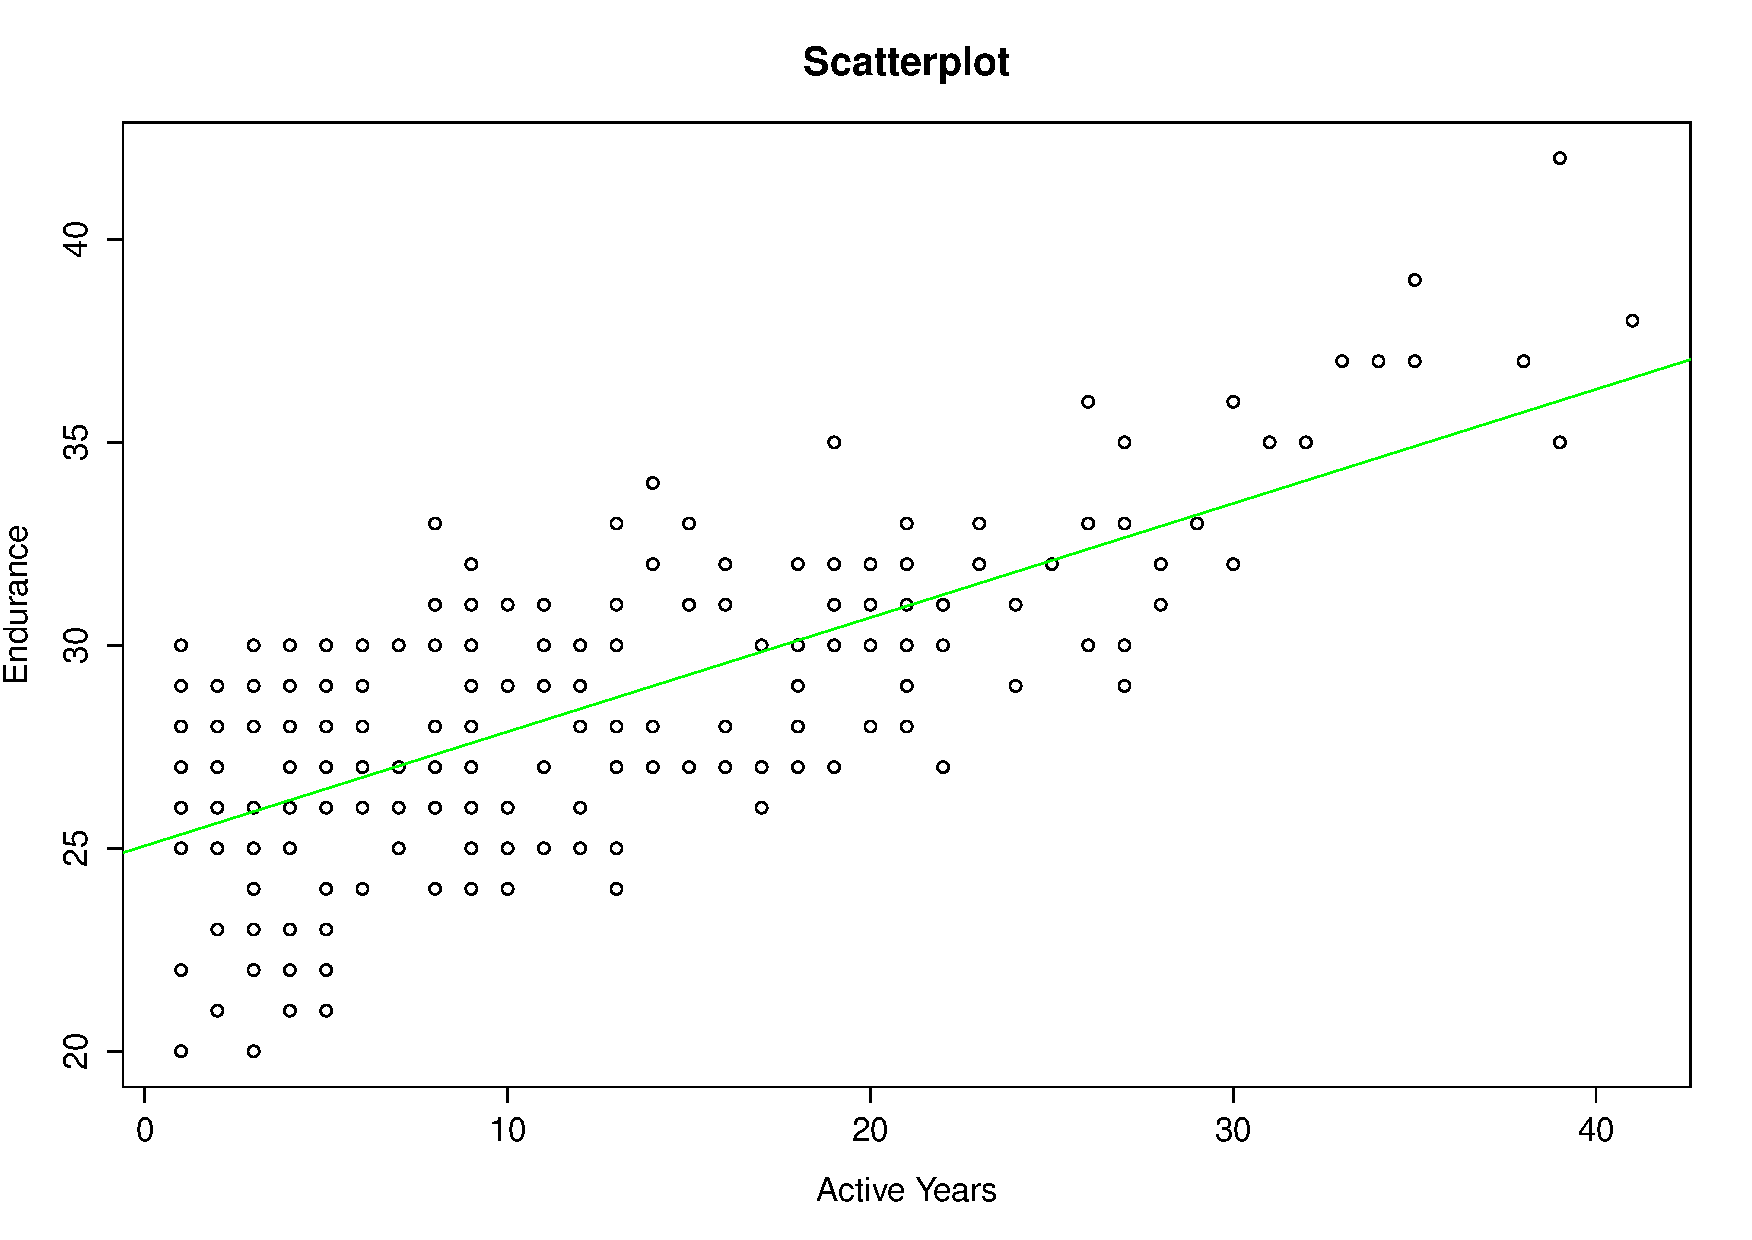
\includegraphics[width=0.9\textheight]{ScatterPlotEnduranceActiveYears}
\end{center}
\end{figure}
\end{frame}


\subsection{Régression linéaire multiple}

\begin{frame}
\frametitle{Régression linéaire multiple (=Modèle linéaire)}
\begin{itemize}
\item La fonction de régression est $r(\truebeta,\bx_i) = \bx_i^T \truebeta$.
On observe
$$(\bx_1,Y_1),\ldots, (\bx_n,Y_n)$$
avec
$$\boxed{Y_i = \bx_i^T \truebeta+ \sigma \xi_i,\;\;i=1,\ldots, n}$$
où $\truetheta \in \Theta = \R^k,\;\;\bx_i \in \R^k$.
\item \alert{Matriciellement}
$$\boxed{\bY = \regressmat\truebeta + \sigma \bnoise}$$
avec
\begin{itemize}
\item \alert<1>{$\bY = (Y_1 \cdots Y_n)^T$},
\item \alert<2>{$\bnoise = (\xi_1 \cdots \xi_n)^T$}
\item \alert<3>{$\regressmat$ la matrice $(n\times k)$
dont la $i$-ème ligne est $\regressmat_{i,\cdot}= \bx_i^T$.}
\end{itemize}
\end{itemize}
\end{frame}





%\begin{frame}
%\frametitle{Estimation de $\sigma^2$}
%\begin{itemize}
%\item \alert{Estimation de $\sigma$} (ou $\sigma^2$) à partir des observations
%$$\boxed{Y_i = \truetheta_0\,+\truetheta_1\,x_i+\alert{\sigma}\, \varepsilon_i,\;\;i=1,\ldots,n}$$
%\alert{avec}
%$$\boxed{\E_\truetheta\big[\varepsilon_i\big]=0,\;\E_\truetheta\big[\varepsilon_i^2\big]=1}$$
%\item \underline{Estimateur naturel} de $\sigma^2$ :
%$$\widehat \sigma_n^2 = \frac{1}{n}\sum_{i = 1}^n\big(Y_i-r(\estregress, x_i)\big)^2$$
%\item Somme de variables aléatoires \alert{non indépendantes}.
%\item Difficile de progresser \alert{sans hypothèse supplémentaire}. Si les $\varepsilon_i$ sont i.i.d. ${\mathcal N}(0,1)$, alors \alert{on sait} \og résoudre \fg{} le problème... plus loin.
%\end{itemize}
%\end{frame}





%\subsection{EMV et EMC}

\begin{frame}
\frametitle{EMC en régression linéaire multiple}
\begin{itemize}
\item Estimateur des \alert{moindres carrés} en régression
linéaire multiple : tout estimateur $\estregress$ satisfaisant
$$\sum_{i = 1}^n
\big(Y_i- \bx_i^T \estregress \big)^2 = \min_{\bcurbeta \in \R^k}\sum_{i =
1}^n \big(Y_i- \bx_i^T \bcurbeta\big)^2.$$
\item En notation matricielle :
\begin{align*}
\|\boldsymbol{Y}-\regressmat\estregress\|^2 &=   \min_{\bcurbeta \in \R^k}\|\bY -\regressmat\truebeta\|^2\\
&= \min_{v \in V}\|\boldsymbol{Y}-v\|^2
\end{align*}
o\`u $V=\text{Im}(\regressmat) = \{v\in \R^n: v=\regressmat \bcurbeta, \
\bcurbeta \in \R^k\}$. \alert{Projection orthogonale sur $V$}.
\end{itemize}
\end{frame}

% \subsection{Géometrie de l'EMC}

 \begin{frame}
\frametitle{Géométrie de l'EMC}
 \begin{itemize}
 \item L'EMC vérifie
$$\boxed{\regressmat \estregress = P_V \boldsymbol{Y}}$$
o\`u $P_V$ est le projecteur orthogonal sur $V$.
\item Comme $ \bY - P_V \bY \perp V$, on en déduit \alert{les équations normales des
moindres carrés}:
$$\boxed{\regressmat^T\regressmat {\estregress} =
\regressmat^T\boldsymbol{Y}.}$$
\item \underline{Remarques.}
  \begin{itemize}
  \item L'EMC est un $Z$-estimateur.
  \item \alert{unicité} de $\estregress$ si la matrice de Gram
  $\regressmat^T\regressmat$ est inversible (la matrice $\regressmat$ est de rang complet).
  \end{itemize}
\end{itemize}
\end{frame}

\begin{frame} \frametitle{Géométrie de l'EMC}
\begin{prop}
Si $\regressmat^T\regressmat$ (matrice $k \times k$) inversible, alors
$\estregress$ \alert{est unique} et
$$\boxed{\estregress = \big(\regressmat^T\regressmat\big)^{-1}\regressmat^T \boldsymbol{Y}}= \regressmat^{\#} \bY$$
\end{prop}
\only<1>{Contient le cas précédent de la droite de régression simple.}
\only<2>{Résultat géometrique, \alert{non stochastique}.
$\regressmat^T\regressmat\ge0$; \ \ $\regressmat^T\regressmat$
inversible $\Longleftrightarrow$ $\regressmat^T\regressmat>0$;
$$\regressmat^T\regressmat>0 \ \Longleftrightarrow \ {\rm rang}(\regressmat)=k
\ \Longleftrightarrow \ {\rm dim}(V)=k.$$
$$\regressmat^T\regressmat>0 \quad \Longrightarrow \quad \alert{ n \geq k}.$$}
\end{frame}


\begin{frame} \frametitle{Géométrie de l'EMC}
Supposons $\regressmat^T\regressmat>0$. Alors, la matrice $n\times n$
$$
\projX = \regressmat\big(\regressmat^T\regressmat\big)^{-1}\regressmat^T = \regressmat \regressmat^{\#}
$$
est dite \alert{matrice chapeau} (\texttt{hat matrix}).
%
\begin{prop}
Si $\regressmat^T\regressmat>0$, alors $\projX$ est le projecteur sur
$V$: \alert{$\projX=P_V$} et \alert{${\rm rang}(\projX)=k$}.
\end{prop}
\only<1>
{\begin{proof}
  $\projX=\projX^T$, $\projX=\projX^2$, donc $\projX$ est un
projecteur. ${\rm Im}(\projX) = V$, donc $\projX=P_V$; \
${\rm rang}(P_V)={\rm dim}(V)=k$.
\end{proof}}
\only<2>
{\alert{Chapeau}, car $\projX$ génère la prévision de
$\regressmat\truetheta$ notée $\widehat{\boldsymbol{Y}}$ :
$$\widehat{\boldsymbol{Y}}= \regressmat\estregress= \projX\boldsymbol{Y}.$$
}
\end{frame}

\begin{frame}
\frametitle{Pseudo-inverse de Moore-Penrose}
Soit $\regressmat$ une matrice $n \times p$ avec $ p \leq n$. On suppose que $\regressmat$ est de rang $p$.
\begin{itemize}
\item $\regressmat^{\#}= (\regressmat^T \regressmat)^{-1} \regressmat^T$ est la \alert{pseudo-inverse} de Moore-Penrose. 
\item $\regressmat^{\#} \regressmat= Id_{p \times p}$: $\regressmat$ est un inverse à gauche de la matrice $\regressmat$.
\item  $\regressmat \regressmat^{\#} = \regressmat (\regressmat^T \regressmat)^{-1} \regressmat^T$ est le projecteur sur l'espace image (l'espace vectoriel engendré par les colonnes de $\regressmat$).
\item Méthode de calcul: décomposition QR ou décomposition en valeurs singulières.
\end{itemize}
\end{frame}

\subsection{Propriétés de l'estimateur des Moindres Carrés}

\begin{frame}
\frametitle{Hypothèses}
\[
\bY= \regressmat \truebeta + \sigma \bnoise
\]
\begin{enumerate}
\item \alert<1>{$\regressmat$ est de rang complet.}
\item \alert<2>{$\PE_\truetheta[\bnoise]= 0$ pour tout $\truetheta \in \Theta$  (les erreurs sont centrées)}
\item \alert<3>{La variance des erreurs est constante et les erreurs sont décorrélées $\PE_{\truetheta}[\bnoise \bnoise^T] = I$ (homoscédasticité)}
\end{enumerate}
\end{frame}

\begin{frame}
\frametitle{Estimateur sans biais}
\begin{theo}
L'estimateur $\estregress$ est sans biais, \ie\ pour tout $\truetheta \in \Theta$, 
\begin{itemize}
\item \PE_{\truetheta}[\estregress]= \truetheta 
\item $\PCov_{\truetheta}(\estregress)= \sigma^2 (\regressmat^T \regressmat)^{-1}$.
\end{itemize}
\end{theo}
\alert{$\estregress = \regressmat^{\#} \bY= \truebeta + \regressmat^{\#} \bnoise$.}
\only<1>{
\begin{align*}
\E_{\truetheta}[\estregress]&=\truebeta + \regressmat^{\#} \PE_{\truetheta}[\bnoise] \\
&= \truebeta
\end{align*}
}
\only<2>{$\estregress- \truebeta= \regressmat^{\#} \bnoise$ ce qui implique
\begin{align*}
\PCov_{\truetheta}(\estregress) &= \E_{\truetheta}\big[ \{\regressmat^{\#} \bnoise \} \{\regressmat^{\#} \bnoise \}^T \big] \\
&= \sigma^2 \{ \regressmat^{\#} \} \{\regressmat^{\#} \}^T = \sigma^2 \big(\regressmat^T\regressmat\big)^{-1}.
\end{align*}
}
\end{frame}

\begin{frame}
\frametitle{Erreur de prédiction}
\begin{itemize}
\item \alert{Erreur de prédiction}:
\begin{align*}
\errpred
&= \bY - \regressmat \estregress= \bY - \regressmat (\regressmat^T \regressmat)^{-1} \regressmat \bY \\
&= (I - \projX) \bY
\end{align*}
\item Sous $\PP_\truetheta$, $\bY= \regressmat \truebeta +  \sigma \bnoise$. Donc,
\begin{align*}
\errpred &= (I-\projX) \regressmat \truebeta + \sigma (I-\projX)  \bnoise \\
         &= \sigma (I-\projX) \bnoise
\end{align*}
car $\projX \regressmat= \regressmat$ ($\projX$ is the orthogonal projector on the image of $\regressmat$).
\end{itemize}
\end{frame}

\begin{frame}
\frametitle{Résidus et variance résiduelle}
\begin{theorem}
Pour tout $\truetheta \in \Theta$
\begin{enumerate}
\item  \alert<1>{$\PE_{\truetheta}[\errpred] = 0$}.
\item  \alert<2>{$\PCov_{\truetheta}(\errpred)= \sigma^2 (I - \projX)$}.
\item  \alert<3>{$\PE_{\truetheta}[\predY]= \regressmat \truebeta$}.
\item  \alert<4>{$\PCov_{\truetheta}(\errpred,\predY)= 0$}.
\end{enumerate}
\end{theorem}
\begin{proof}
\only<1> {
\begin{align*}
\PE_{\truetheta}[\errpred] &= \sigma \PE_{\truetheta}[ (I-\projX) \bnoise] \\
&= \sigma (I-\projX) \PE_{\truetheta}[\bnoise] \eqsp.
\end{align*}
}
\only<2> {
\begin{align*}
\PCov_{\truetheta}(\errpred)&= \sigma^2 (I-\projX) \PE_{\truetheta}[\bnoise \bnoise'] (I- \projX) \\
&= \sigma^2 (I-\projX).
\end{align*}
}
\only<3> {
\begin{align*}
\PE_{\truetheta}[\predY] &= \PE_{\truetheta}[ \projX (\regressmat \truebeta + \sigma \bnoise)] \\
&=  \projX \regressmat \truebeta + \sigma \PE_{\truetheta}[ \bnoise] \\
&= \regressmat \truebeta.
\end{align*}
}
\only<4>{
On a $\predY - \PE_{\truetheta}[\predY]= \sigma \projX \bnoise$ et donc
\begin{align*}
\PCov_{\truetheta}(\errpred,\predY) &= \sigma^2 \PE_{\truetheta}[ (I-\projX) \bnoise \bnoise' \projX] \\
&= \sigma^2 (I- \projX) \projX= 0.
\end{align*}
}
\end{proof}
\end{frame}



\begin{frame}
\frametitle{Estimateur sans biais de la variance de l'erreur de prédiction}
\begin{theo}
$\hat{\sigma}_n^2= (n-p)^{-1} \| \errpred \|^2$ est un estimateur sans biais de la variance de l'erreur.
\end{theo}
\begin{proof}
Comme $(I-\projX)^2= (I-\projX)$, nous avons
\begin{align*}
\PE_{\truetheta}[\hat{\sigma}_n^2] &= (n-p)^{-1} \PE_{\truetheta}[ \bnoise^T (I-\projX) \bnoise] \\
                             &= (n-p)^{-1} \PE_{\truetheta}[ \mathrm{Tr}( (I-\projX) \bnoise \bnoise) ] \\
                             &= \sigma^2 (n-p)^{-1} \mathrm{Tr}(I-\projX)= \sigma^2 \eqsp.
\end{align*}
\end{proof}
\end{frame}

\begin{frame}
\frametitle{Coefficient de détermination}
\begin{itemize}
\item \alert{Pythagore} 
\begin{align*}
\| \bY \|^2 &= \| \projX \bY \|^2 + \| (I - \projX) \bY \|^2 \\
            &= \| \predY \|^2 + \| \errpred \|^2
\end{align*}
\item \alert{Coefficient de détermination}
\begin{align*}
R^2 &= \frac{\|\bY\|^2}{\|\bY\|^2} 
    &= 1 - \frac{\| \errpred \|^2}{\|\bY\|^2} = 1 - \frac{\mathrm{SCR}}{\mathrm{SCT}}
\end{align*}
où \alert{SCR} est la somme des carrés résiduels (RSS: residual sum of squares) et \alert{SCT} est la somme des carrés totaux.
\end{itemize}
\end{frame}

\begin{frame}
\frametitle{Coefficient de détermination}
Lorsque le vecteur constant est incluse dans la matrice de régression, on retranche aux observations leurs moyennes. 
\begin{itemize}
\end{itemize}
\end{frame}




\begin{frame}
\frametitle{Diagnostic de régression}
\begin{figure}
  \centering
  % Requires \usepackage{graphicx}
  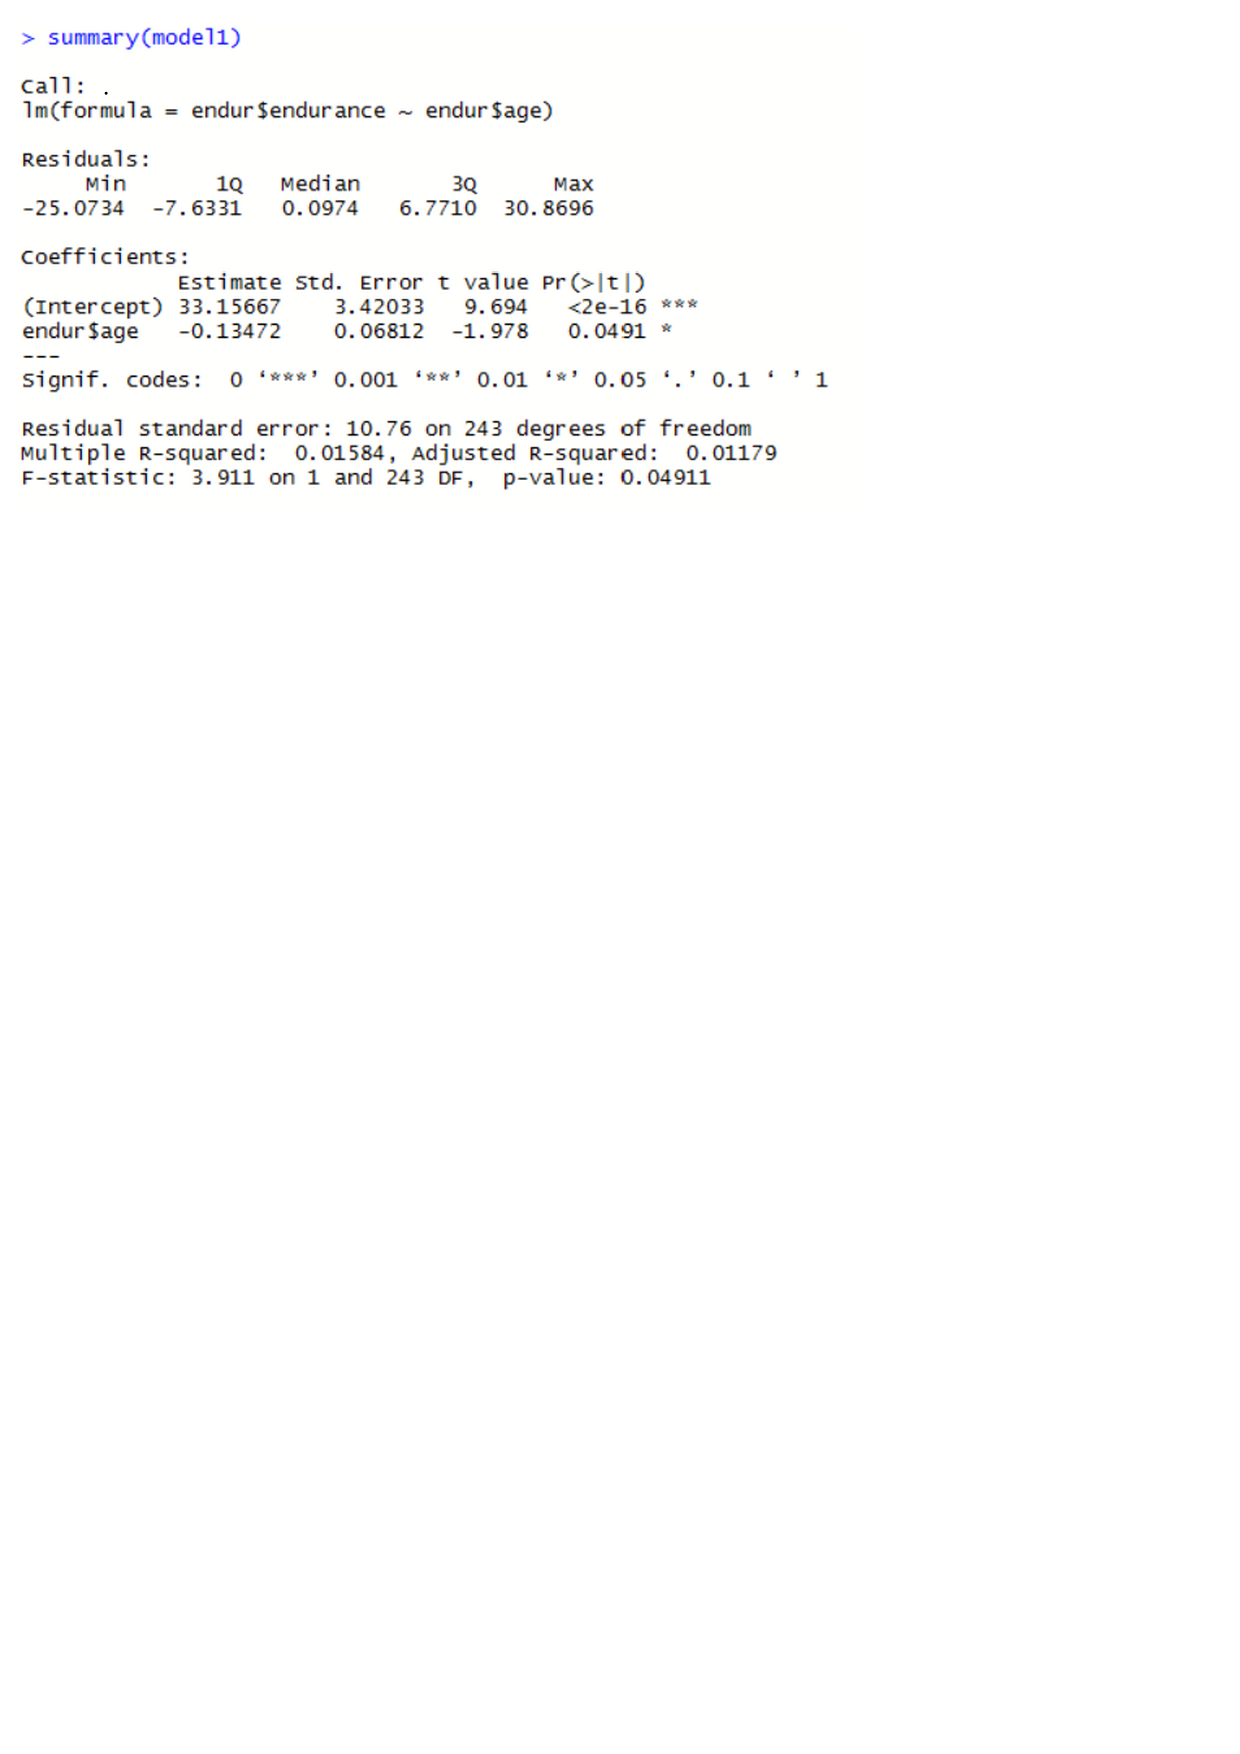
\includegraphics[width=0.6\textwidth]{summarymodel1}\\
  \caption{Régression à un facteur: endurance / âge}
\end{figure}
\end{frame}


\begin{frame}
\frametitle{Diagnostic de régression}
\begin{figure}
  \centering
  % Requires \usepackage{graphicx}
  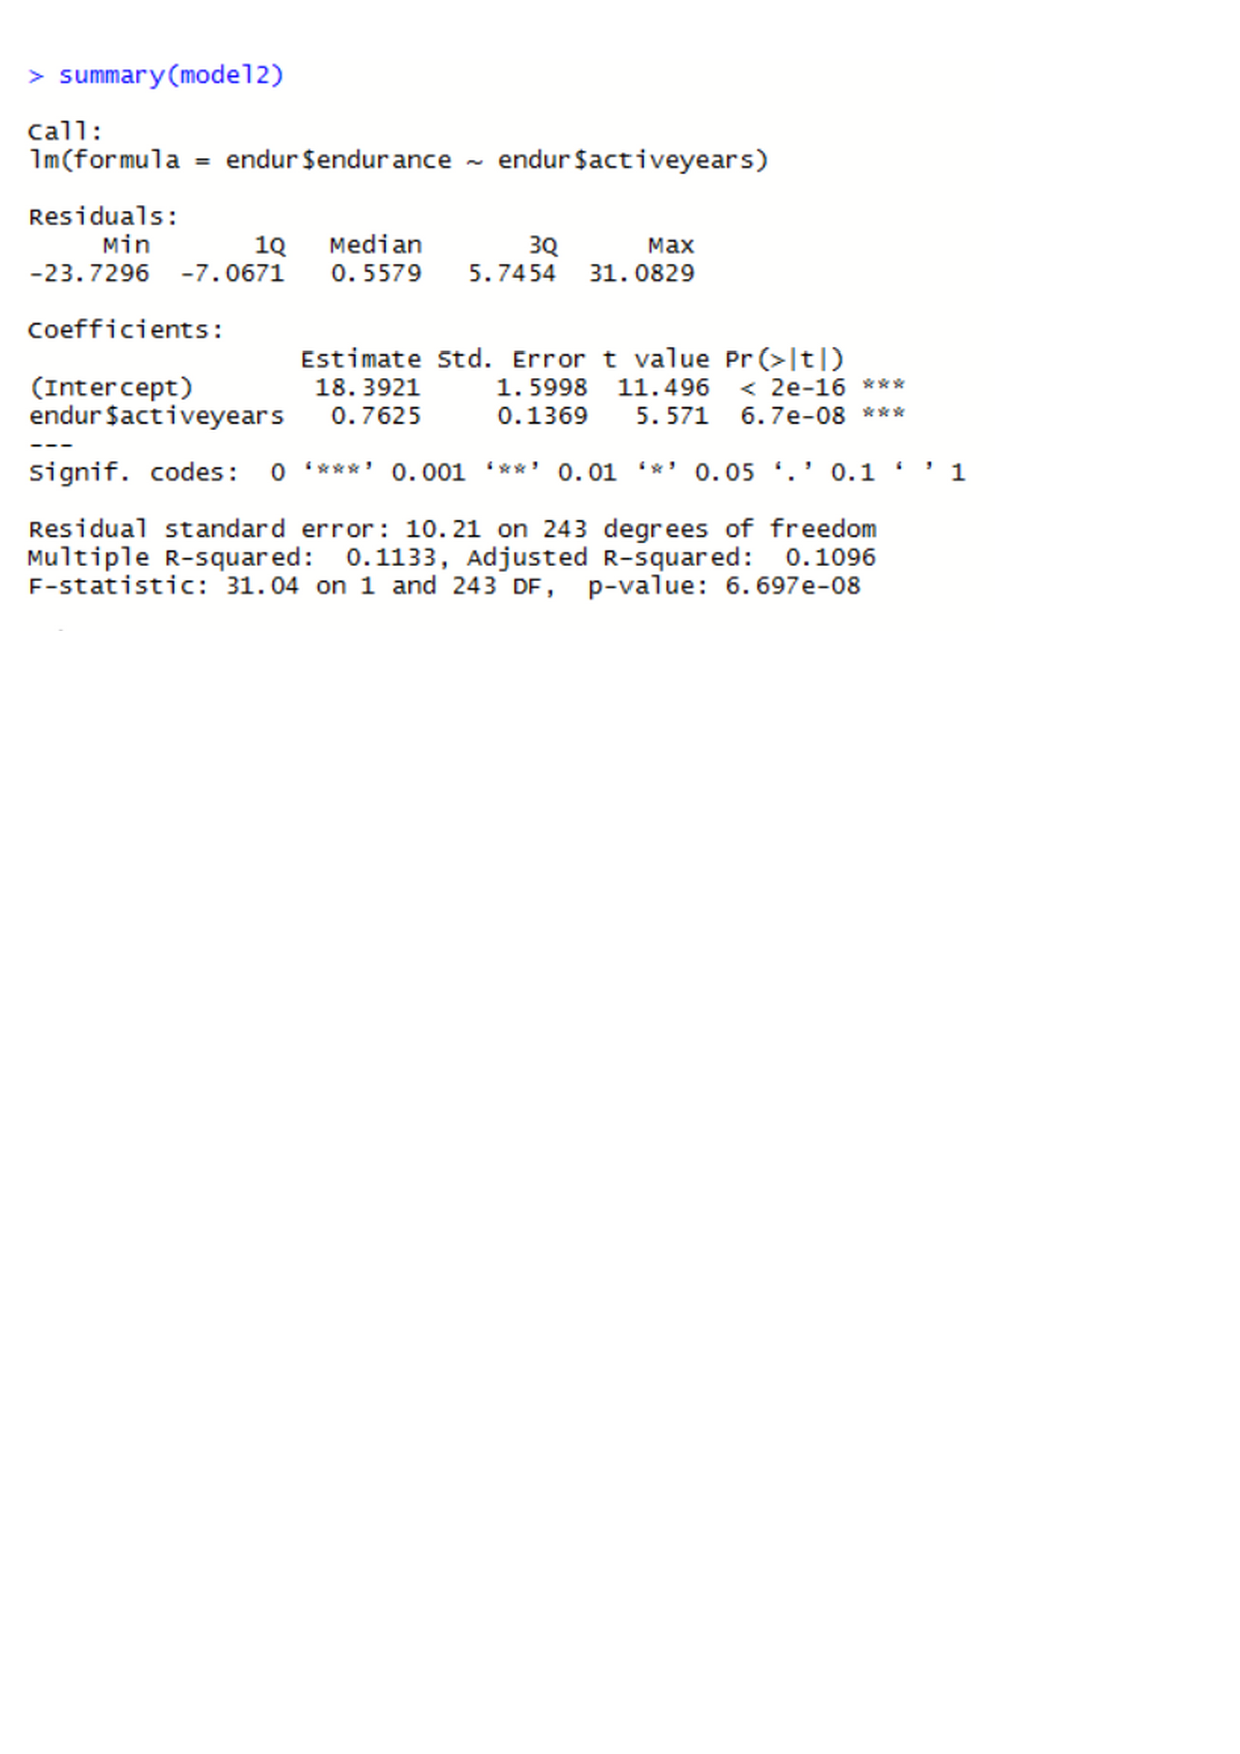
\includegraphics[width=0.6\textwidth]{summarymodel2}\\
  \caption{Régression à un facteur: endurance / nombre d'années de pratique}
\end{figure}
\end{frame}

\begin{frame}
\frametitle{Diagnostic de régression}
\begin{figure}
  \centering
  % Requires \usepackage{graphicx}
  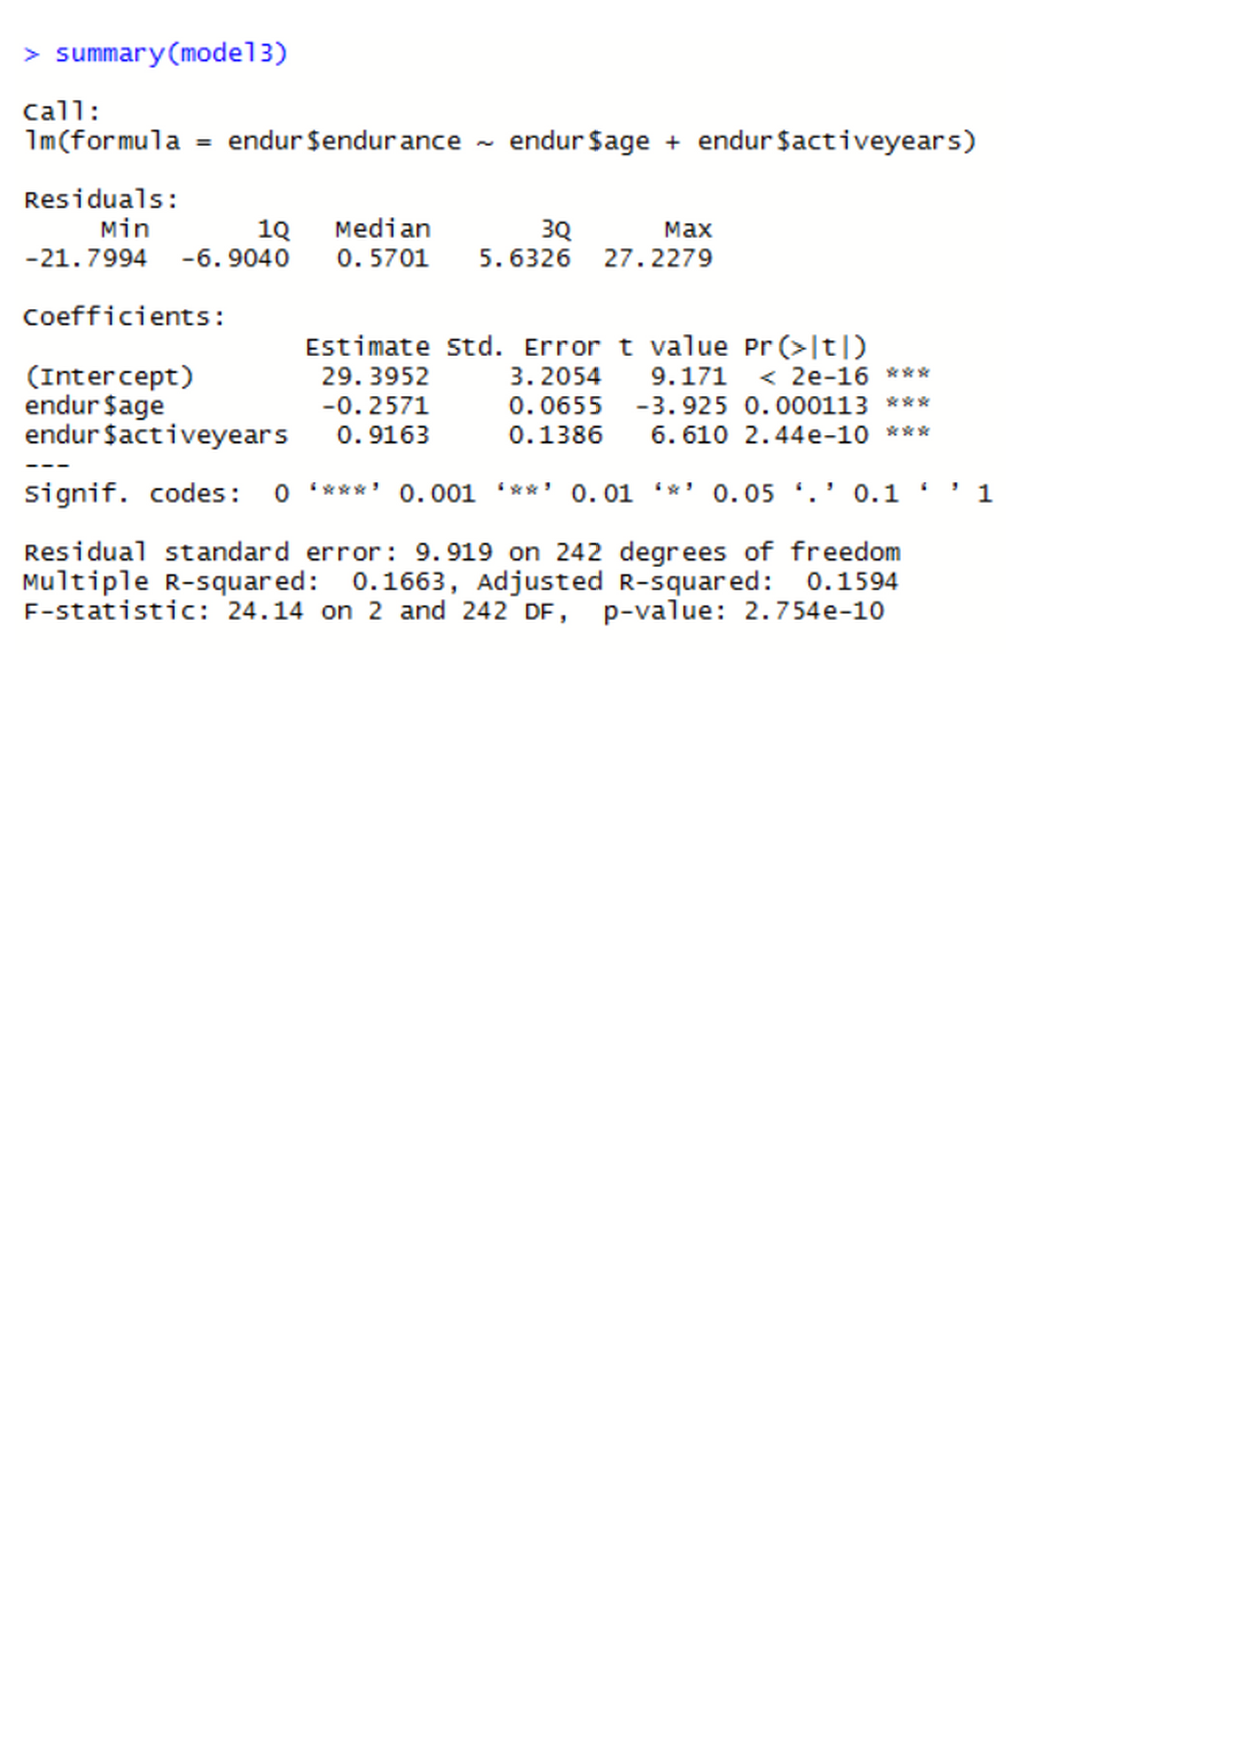
\includegraphics[width=0.6\textwidth]{summarymodel3}\\
  \caption{Régression à un deux facteurs: endurance / âge + nombre d'années de pratique}
\end{figure}
\end{frame}








\subsection{Modèle linéaire gaussien}

\begin{frame}
\frametitle{Régression gaussienne} \alert{Régression gaussienne} : on
suppose $\bnoise \sim {\mathcal N}(0,\mathrm{Id}_n)$. Alors on a plusieurs proriétés
remarquables:
\begin{itemize}
\item  On sait expliciter la loi \alert{ exacte} (non-asymptotique!)
de~$(\estregress,\hat{\sigma}^2)$.\\\vspace{1mm} 
\item \alert{Ingrédient} : 
\begin{itemize}
\item loi des vecteurs gaussiens sont caractérisés par leur moyenne et matrice de
variance-covariance.
\item pour des vecteurs gaussiens, la décorrélation implique l'indépendance.
\end{itemize}
\end{itemize}
\end{frame}

%\subsection{Propriétés statistiques de l'EMC : cas gaussien}

\begin{frame}
\frametitle{Cadre gaussien : loi des estimateurs}
\begin{prop}
\begin{enumerate}
\item  $\estregress \sim {\mathcal N}\big(\truebeta, \sigma^2 \big(\regressmat^T\regressmat\big)^{-1}\big)$
\item  $\|(I - \projX) \bY \|^2 \sim
\sigma^2\chi^2(n-k)$ \alert{ loi du Chi 2 à $n-k$ degrés de liberté}
\item  $\estregress$ et $(I - \projX) \bY$ sont indépendants.
\end{enumerate}
\end{prop}
\end{frame}

\begin{frame}
\frametitle{Théorème de Cochran}
\begin{theo}
Soit $\bY \sim N(\mu,\sigma^2 I_n)$, $\mathcal{M}$ un sous espace de $\R^n$ de dimension $k$, $\Pi$ la matrice de projection orthogonale 
sur $\mathcal{M}$ et $\Pi_{\perp}= I_n - \Pi$ la matrice de projection orthogonale sur $\mathcal{M}^\perp$. Nous avons
\begin{enumerate}
\item \alert<1> $\Pi \bY \sim N(\Pi \mu, \sigma^2 \Pi)$, $\Pi_\perp \bY \sim N(\Pi_\perp \mu, \sigma \Pi_\perp)$
\item \alert<2> les vecteurs $\Pi \bY$ et $\Pi_\perp \bY$ sont indépendants
\item \alert<3> $\| \Pi(\bY - \mu) \|^2 / \sigma^2 \sim \chi^2_k$ et $\Pi_\perp(\bY-\mu) \|^2/\sigma^2 \sim \chi^2_{n-k}$.
\end{enumerate}
\end{theo}
\end{frame}

\begin{frame}
\frametitle{Cadre gaussien : loi des estimateurs}
\begin{prop}
\begin{enumerate}
\item  \alert<1>{$\estregress \sim {\mathcal N}\big(\truebeta, \sigma^2 \big(\regressmat^T\regressmat\big)^{-1}\big)$}
\item  \alert<2>{$\|(I - \projX) \bY \|^2 \sim
\sigma^2\chi^2(n-k)$ loi du Chi 2 à $n-k$ degrés de liberté}
\item  \alert<3>{$\estregress$ et $(I - \projX) \bY$ sont indépendants}.
\end{enumerate}
\end{prop}
\only<1>{
\begin{itemize}
\item Définition: $\estregress= \regressmat^{\#} \bY$ et $\bY \sim N(\regressmat \truebeta, \sigma^2 I_n)$. 
\item   $\estregress \sim N(\regressmat^{\#} \regressmat \truebeta, \sigma^2 \{ \regressmat^{\#} \} \{ \regressmat^{\#} \}^T)$ 
\item On conclut en remarquant $\regressmat^{\#} \regressmat= I_k$ et
$\{ \regressmat^{\#} \} \{ \regressmat^{\#} \}^T = (\regressmat^T \regressmat)^{-1}$
\end{itemize}}
\only<2>{Application directe de Cochran en remarquant que 
$$
(I-\projX) \PE_{\truetheta}[\bY] = (I - \projX) \bX \true \beta = 0.
$$
}
\only<3>{
\begin{itemize}
\item Le théorème de Cochran montre que $\projX \bY$ et $(I-\projX) \bY$ sont indépendants. 
\item On conclut en remarquant que $\estregress= \regressmat^{\#} \bY = \regressmat^{\#} \projX \bY$. 
\end{itemize}
}
\end{frame}




\begin{frame}
\frametitle{Estimateur de la variance $\sigma^2$: cadre gaussien}
$$\boxed{\widehat \sigma_n^2 = \frac{\| (I-\projX) \bY \|^2}{n-\alert{k}} = \frac{1}{n-\alert{k}}\sum_{i = 1}^n\big(Y_i-\bx_i^T \estregress \big)^2}$$
D'après la dernière Proposition :
\begin{itemize}
\item $\widehat
\sigma_n^2/\sigma^2 \sim \chi^2(n-k)$ \alert{ loi du Chi 2 à
$n-k$ degrés de liberté}
\item C'est un estimateur \alert{sans biais}: $$\E_\truetheta\big[\widehat
\sigma_n^2\big]=\sigma^2.$$
\item $\widehat
\sigma_n^2$ est \alert{indépendant} de $\estregress$.
\end{itemize}
\end{frame}

\begin{frame}
\frametitle{Lois des coordonnées de $\estregress$: cadre gaussien}
\begin{itemize}
\item :
$$
(\estregress)_j -\truetheta_j \sim {\mathcal N}\big(0, \sigma^2 b_j)
$$
o\`u $b_j$ est le $j$ème élément diagonal de $\big(\regressmat^T
\regressmat\big)^{-1}$. $$ \frac{(\estregress)_j -\truetheta_j}{\widehat
\sigma_n \sqrt{b_j}} \sim t_{n-k}$$ \alert{loi de Student \`a
$n-k$ degrés de liberté}.
$$ t_q = \frac{\xi}{\sqrt{\eta/q}}$$
o\`u $q\ge 1$ un entier, $\xi\sim {\mathcal N}\big(0,1)$, $\eta\sim
\chi^2(q)$ et\\ $\xi$ \alert{indépendant} de $\eta$.
\end{itemize}
\end{frame}

\begin{frame}
    \frametitle{Exemple de données de régression}
\begin{figure}
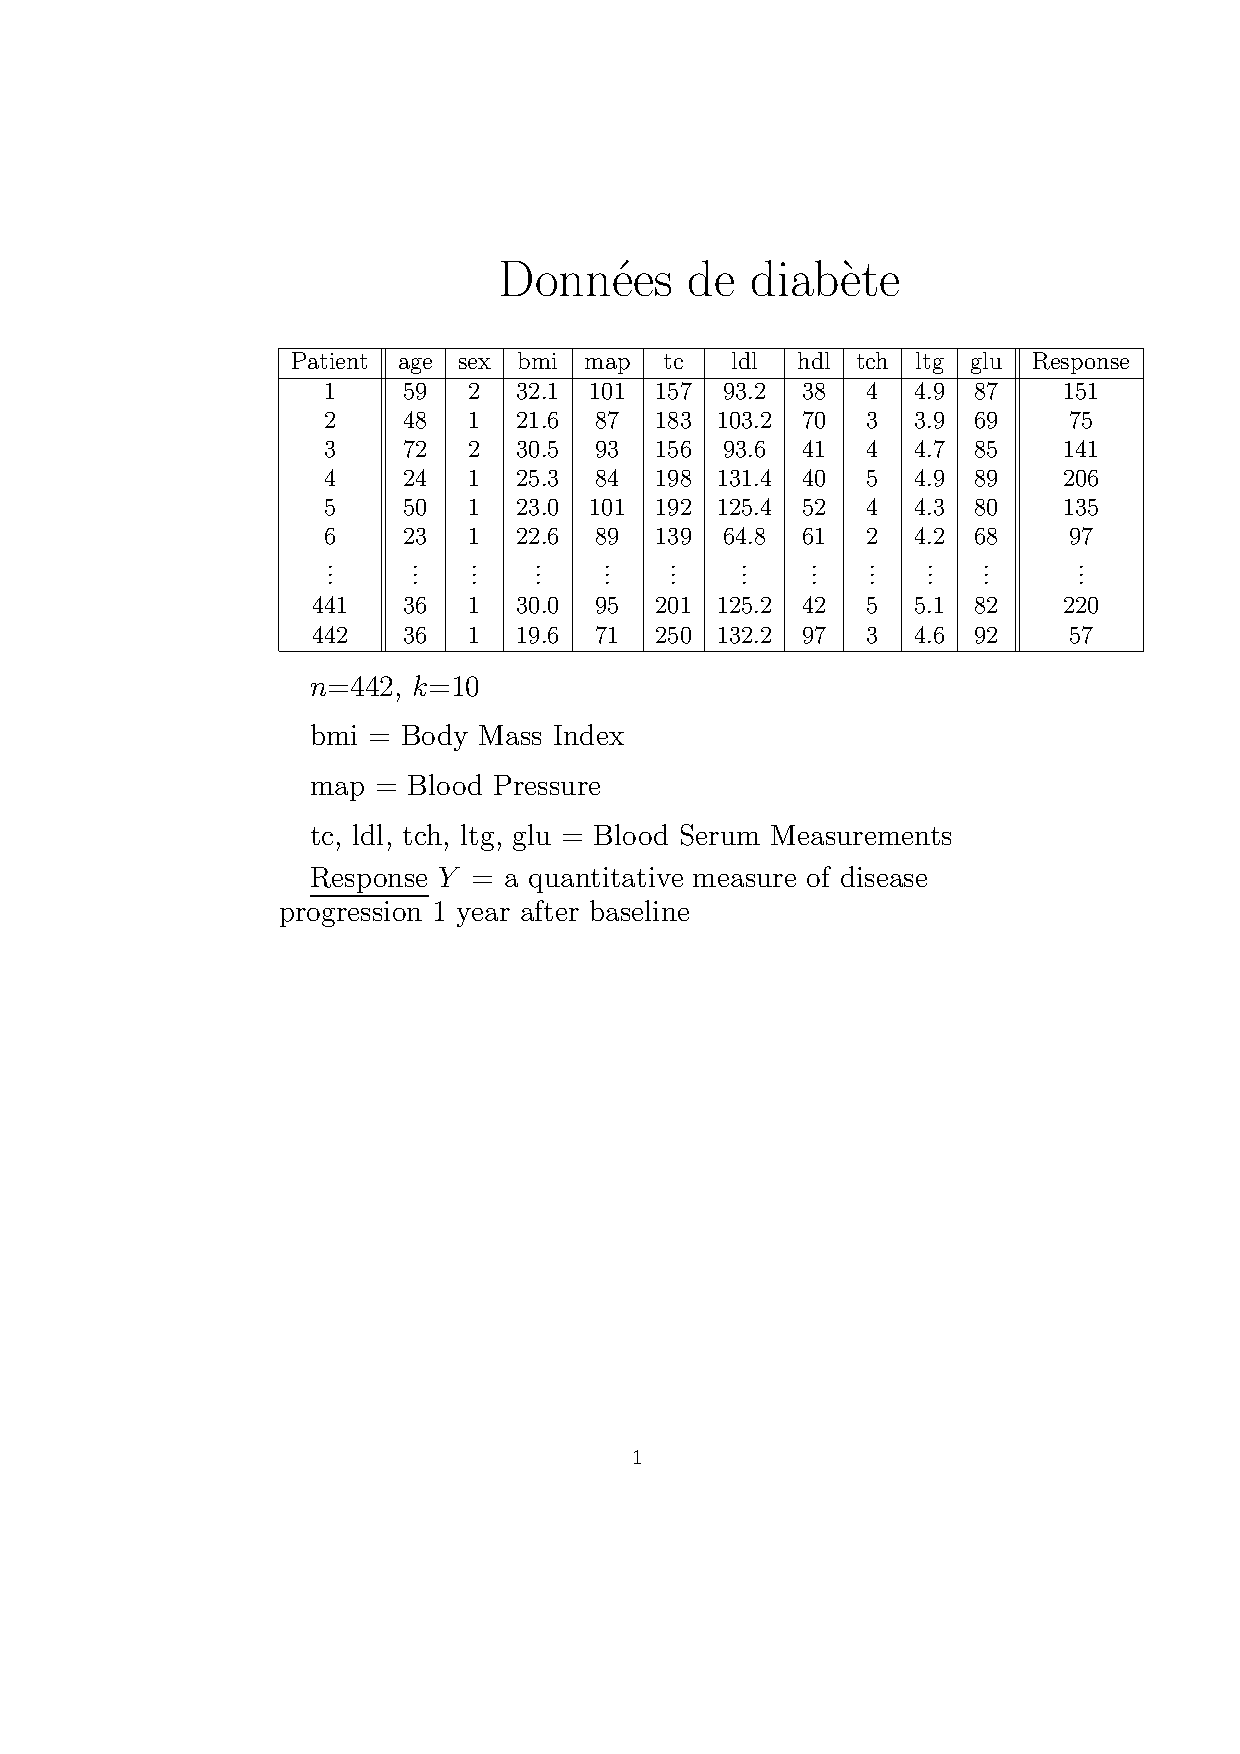
\includegraphics[height=2\textheight]{cours4_data1}
\end{figure}
\end{frame}

\begin{frame}
\frametitle{Résultats de traitement statistique initial}
\begin{tabular}{|c||c|c|c|c|}
\hline &Estimate&Std. Error&t value&Pr($>|t|$)\\\hline
(Intercept) &$152.133$&$2.576$&$59.061$&$< 2e-16***$\\
age&$-10.012$&$59.749$&$ -0.168$&$0.867000$\\\hline
sex &$-239.819$&$61.222$&$-3.917$&$0.000104***$\\
bmi&$519.840$&$66.534$&$7.813$&$4.30e-14***$\\\hline
map&$324.390$&$65.422$&$4.958$&$1.02e-06***$\\
tc&$-792.184$&$416.684$&$-1.901$&$0.057947$\\\hline
ldl&$476.746$&$339.035$&$1.406$&$0.160389$\\
hdl&$101.045$&$212.533 $&$0.475$&$0.634721$\\\hline
tch&$177.064$&$161.476$&$ 1.097$&$0.273456$\\
ltg&$751.279$&$ 171.902$&$4.370$&$ 1.56e-05***$\\\hline
glu&$67.625$&$ 65.984$&$1.025$&$0.305998$\\\hline
\end{tabular}
\end{frame}

\begin{frame}
\frametitle{Questions statistiques}
\begin{itemize}
\item \alert{Sélection de variables.} Lesquelles parmi les 10
variables:\\\vspace{3mm}
\centerline{\texttt{age,sex,bmi,map,tc,ldl,hdl,tch,ltg,glu}}\vspace{3mm}
sont significatives? Formalisation mathématique: trouver (estimer)
l'ensemble $N= \{j: \truetheta_{j}\ne 0\}$.
\item \alert{Prévison.} Un nouveau patient arrive avec son vecteur
des 10 variables $\alert{x}_0\in \R^{10}$. Donner la prévison de la
réponse $Y$ =état du patient dans 1 an.
\end{itemize}
\end{frame}

\section{Sélection de variables}

\begin{frame}
\frametitle{RSS (Residual Sum of Squares)} Modèle de
régression\vspace{2mm} \centerline{$ Y_i= r(\truetheta, {\bf
x}_i)+\xi_i, \quad i=1,\dots,n.$}
\begin{itemize}
\item \alert{Résidu:} si $\est$ est un estimateur de
$\truetheta$,
$$\widehat \xi_i = Y_i - r(\est, \alert{x}_i)
\;\;\text{\alert{résidu} au point}\;i.$$
\item \alert{RSS:} \alert{ Residual Sum of Squares}, somme
résiduelle des carrés. Caractérise la qualité
d'approximation.
$${\rm RSS}(={\rm RSS}_{\est})=\|\widehat \xi\|^2
= \sum_{i = 1}^n\big(Y_i - r(\est,\alert{x}_i)\big)^2.$$
\item En régression \alert{linéaire}:
$\boxed{{\rm RSS}= \|\alert{Y}-\regressmat\est\|^2.}$
\end{itemize}
\end{frame}


%\section{Prévision}

\begin{frame}
\frametitle{Prévision}

Modèle de régression \vspace{2mm} \centerline{$ Y_i=
r(\truetheta, \alert{x}_i)+\xi_i, \quad i=1,\dots,n.$} Régression
\alert{linéaire}: $r(\truetheta, \alert{x}_i)=\truetheta^T{\bf
x}_i$. Exemple: $\alert{x}_i$ vecteur de 10 variables explicatives
(\texttt{age,sex,bmi,...}) pour patient $i$.
\begin{itemize}
\item \alert{Problème de prévision}:
Un nouveau patient arrive avec son vecteur des 10 variables ${\bf
x}_0\in \R^{10}$. Donner la prévison de la valeur de fonction de
régression $r(\truetheta, \alert{x}_0)=\truetheta^T\alert{x}_0$\\
(=état du patient dans 1 an).
\item Soit $\est$ un estimateur de $\truetheta$. \alert{Prévision par
substitution:}
 \centerline{$\boxed{ \widehat Y = r(\est, \alert{x}_0).}$}
\item \underline{Question statistique}: quelle est la qualité de la prévision?
\alert{Intervalle de confiance} pour $r(\truetheta, \alert{x}_0)$
basé sur $\widehat Y$?
\end{itemize}
\end{frame}


\section{Prévision}
\begin{frame}
\frametitle{Prévision}
\begin{itemize}
\item Un des buts de la régression est de proposer des prédictions pour la réponse lorsque nous avons de
nouvelles valeurs des variables explicatives.
\item Un prédicteur naturel de la réponse est \alert{$\hat{Y}_n(\bx)= \bx^T \estregress$}
\end{itemize}
\end{frame}

\begin{frame}
\frametitle{Moyenne et variance de la prévision}
\begin{theorem}
\begin{itemize}
\item $\PE_{\truetheta}[\hat{Y}_n(\bx)]= \bx^T \truebeta$
\item $\Var_{\truetheta}(\hat{Y}_n(\bx))= \sigma^2 \bx^T (\regressmat^T \regressmat)^{-1} \bx$
\item $\PE_{\truetheta}[ (Y(\bx) - \hat{Y}_n(\bx))^2]= \sigma^2 (1 + \bx' (\regressmat^T \regressmat)^{-1} \bx)$
\end{itemize}
\end{theorem}
\only<1>{$\hat{Y}_n(\bx)= \bx^T \estregress$ et $\PE_{\truetheta}[\estregress]= \truebeta$}
\only<2>{
\begin{align*}
\hat{Y}_n(\bx)- \bx^T \truebeta
&= \bx^T (\regressmat^T \regressmat)^{-1} \regressmat^T \bY - \bx^T \truebeta \\
&= \bx^T (\regressmat^T \regressmat)^{-1} \regressmat^T (\regressmat \truebeta + \sigma \bnoise) - \bx^T \truebeta \\
&= \sigma \bx^T (\regressmat^T \regressmat)^{-1} \regressmat^T \bnoise
\end{align*}}
\only<3>{
\begin{align*}
\PE_{\truetheta}[ (Y(\bx) - \hat{Y}_n(\bx))^2]
&= \PE_{\truebeta}[ (Y(\bx) - \PE_{\truebeta}[\hat{Y}_n(\bx)])^2] + \Var_{\truetheta}(\hat{Y}_n(\bx)) \\
&= \PE_{\truebeta}[ (Y(\bx) - \bx^T \truebeta)^2] +  \sigma^2 \bx^T (\regressmat^T \regressmat)^{-1} \bx
\end{align*}
}
\end{frame}


\begin{frame}
\frametitle{Prévision: modèle linéaire gaussienne}
\begin{itemize}
\item Traitement sur l'exemple: $r(\truetheta, \alert{x})=\truetheta^T{\bf
x}$, régression \alert{linéaire gaussienne} et $\boxed{\widehat Y = {\bf
x}_0^T\estregress}$
\item \underline{Hyp. 1} : $\bnoise \sim {\mathcal N}(0,\sigma^2\mathrm{Id}_n)$.
\item \underline{Hyp. 2} : $\regressmat^T \regressmat>0$.
\end{itemize}
\begin{prop}
\begin{itemize}
\item[(i)] $\widehat Y \sim {\mathcal N}\big({\bx_0^T\truebeta, \sigma^2 {\bf
x}_0^T\big(\regressmat^T\regressmat\big)^{-1}\alert{x}_0\big)$
\item[(ii)] $\widehat Y- \bx_0^T\truebeta$ et $\bY-\regressmat \estregress$ sont
indépendants.
\end{itemize}
\end{prop}
Rappel: $\|\boldsymbol{Y}-\regressmat \estregress\|^2 \sim
\sigma^2\chi^2(n-k)$ \alert{ loi du Chi 2 à $n-k$ degrés de
liberté}.
\end{frame}

\begin{frame}
\frametitle{Prévision: modèle linéaire gaussienne}
\begin{itemize}
\item D'après la Proposition,
$$
\eta:=\frac{\widehat Y -\alert{x}_0^T\truebeta} {\sqrt{\sigma^2 {\bx_0^T\big(\regressmat^T\regressmat\big)^{-1}\alert{\bx}_0}}\sim {\mathcal
N}(0,1).
$$
\item On replace $\sigma^2$ inconnu par $\widehat \sigma_n^2 =
{\|(I-\projX) \bY \|^2}/({n-k}).$
\item \alert{$t$-statistique:}
$$
t:= \frac{\widehat Y -\alert{\bx}_0^T\truebeta} {\sqrt{\widehat
\sigma_n^2 \alert{\bx}_0^T\big(\regressmat^T\regressmat\big)^{-1}{
\bx_0}}=\frac{\eta}{\sqrt{\chi/(n-k)}}\sim t_{n-k},
$$
\alert{loi de Student à $n-k$ degrés de liberté}, car $\eta\sim
{\mathcal N}(0,1)$, $\chi:=\|\boldsymbol{Y}-\regressmat
\estMC\|^2/\sigma^2\sim \chi^2(n-k)$ et $\eta\ind\chi$.
\end{itemize}
\end{frame}

\begin{frame}
\frametitle{Prévision: intervalle de confiance}
\begin{eqnarray*}
&&\PP \Big(-q_{1-\frac{\alpha}{2}}(t_{n-k}) \le \frac{\widehat Y
-\alert{x}_0^T\truetheta} {\sqrt{\widehat \sigma_n^2 {\bf
x}_0^T\big(\regressmat^T\regressmat\big)^{-1}\alert{x}_0}}\le
q_{1-\frac{\alpha}{2}}(t_{n-k})\Big) \\\hspace{4mm} &&= \PP(-
q_{1-\frac{\alpha}{2}}(t_{n-k}) \le t\le
q_{1-\frac{\alpha}{2}}(t_{n-k})) = 1-\alpha.
\end{eqnarray*}
$\Longrightarrow$ \alert{intervalle de confiance} de niveau
$1-\alpha$ pour $r(\truetheta,\alert{x}_0)=\alert{x}_0^T\truetheta$ est
\alert{$[r_L, r_U]$}, o\`u:
\begin{eqnarray*}
\alert{r_L}&=&\widehat Y -
q_{1-\frac{\alpha}{2}}(t_{n-k})\sqrt{\widehat \sigma_n^2
\alert{x}_0^T\big(\regressmat^T\regressmat\big)^{-1}\alert{x}_0},\\
\alert{r_U}&=& \widehat Y +
q_{1-\frac{\alpha}{2}}(t_{n-k})\sqrt{\widehat \sigma_n^2 {\bf
x}_0^T\big(\regressmat^T\regressmat\big)^{-1}\alert{x}_0}.
\end{eqnarray*}
\end{frame}



\begin{frame}
\frametitle{Limites des moindres carrés et du cadre gaussien}
\begin{itemize}
\item Calcul \alert{explicite} (et efficace) de l'EMC  limité à
une fonction de régression \alert{linéaire}.
\item Modèle linéaire donne un cadre assez général:
\begin{itemize}
\item Modèle
polynomial, \item \alert{Modèles avec interactions...}
\end{itemize}
\item \alert{ Hypothèse de gaussianité} = cadre asymptotique implicite.
\item Besoin d'outils pour les modèles  à réponse \alert{$Y$ discrète}.
\end{itemize}
\end{frame}

%\section{Régression linéaire non-gaussienne}

\begin{frame}
\frametitle{Régression linéaire non-gaussienne} Modèle de
régression linéaire \vspace{3mm} \centerline{$ Y_i= \truetheta^T
\alert{x}_i+\xi_i, \quad i=1,\dots,n.$}

\vspace{-2mm}

\begin{itemize}
\item \underline{Hyp. 1'} : \alert{$\xi_i$ i.i.d., $\E[\xi_i]
=0$, $\E[\xi_i^2] = \sigma^2>0$.}
\item \underline{Hyp. 2'} : $\regressmat^T \regressmat>0$, \alert{$\lim_n\max_{1\le i \le n}\alert{x}_i^T
\big(\regressmat^T \regressmat\big)^{-1}\alert{x}_i =0$.}
\end{itemize}
\begin{prop}[Normalité asymptotique de l'EMC]
$$
\sigma^{-1}\big(\regressmat^T
\regressmat\big)^{1/2}(\estMC-\truetheta)\stackrel{d}{\longrightarrow}
{\mathcal N}\big(0, \mathrm{Id}_k), \quad n\to\infty.
$$
\end{prop}
\begin{itemize}
\item A comparer avec le cadre gaussien:\vspace{2mm}
\centerline{$\sigma^{-1}\big(\regressmat^T
\regressmat\big)^{1/2}(\estMC-\truetheta)\sim {\mathcal N}\big(0,
\mathrm{Id}_k)$ \text{pour tout $n$.}}
\end{itemize}
\end{frame}

%\begin{frame}
%\frametitle{Vitesses de convergence}
%\end{frame}

%\subsection{Propriété de l'EMC: cadre général (non-gaussien) }
%
%\begin{frame}
%\begin{itemize}
%\item \underline{Hyp. 1} : $\regressmat^T \regressmat$ inversible
%\item  \underline{Hyp. 2} :
%\alert{$\E\big[\bnoise\big]=0$,
%$\E\big[\bnoise\bnoise^T\big] = \sigma^2
%\mathrm{Id}_n$}.
%\end{itemize}
%\begin{prop}
%%Sous les hypothèses précédentes
%\begin{itemize}
%\item $\E_\truetheta\big[\estMC\big]=\truetheta$ et
%$$\E_\truetheta\big[\big(\estMC-\truetheta\big)\big(\estMC-\truetheta\big)^T\big]=\sigma^2 \big(\regressmat^T\regressmat\big)^{-1}$$
%\item Si l'on pose
%$$\boxed{\widehat \sigma_n^2 = \frac{\|\boldsymbol{Y}-\regressmat \estMC\|^2}{n-\alert{k}} = \frac{1}{n-\alert{k}}\sum_{i = 1}^n\big(Y_i-(\estMC)^T\bx_i\big)^2}$$
%alors $\E_\truetheta\big[\widehat \sigma_n^2\big]=\sigma^2.$
%\end{itemize}
%\end{prop}
%\end{frame}





\section{Régression non-linéaire}


\begin{frame}
\frametitle{Régression non-linéaire}
\begin{itemize}
\item On observe
$$(\bx_1,Y_1),\ldots, (\bx_n,Y_n),$$
où
$$\boxed{Y_i = r(\alert{\truetheta},\bx_i)+\xi_i,\;\;i=1,\ldots,n}$$
avec
$$\bx_i\in \R^k,\;\;\text{et}\;\; \alert{\truetheta \in \Theta \subset \R^d}.$$
\item Si $\xi_i \sim_{\text{i.i.d.}} {\mathcal N}(0,\sigma^2)$,
$${\mathcal L}_n(\truetheta, Y_1,\ldots, Y_n) \propto \exp\Big(-\frac{1}{2\sigma^2}\sum_{i = 1}^n\big(Y_i-r(\truetheta,\bx_i)\big)^2\Big)$$
et l'estimateur du \alert{maximum de vraisemblance} est obtenu en minimisant la fonction
$$\truetheta \leadsto \sum_{i = 1}^n\big(Y_i-r(\truetheta,\bx_i)\big)^2.$$
\end{itemize}
\end{frame}

\begin{frame}
\frametitle{Moindre carrés non-linéaires}
\begin{df}
\begin{itemize}
\item $M$-estimateur associé à la \alert{fonction de contraste} $\psi:\Theta \times \alert{\R^k}\times \R\rightarrow \R$ : tout estimateur $\est$ satisfaisant
$$\sum_{i = 1}^n \psi(\est, \bx_i, Y_i) = \max_{a \in \Theta} \sum_{i = 1}^n \psi(a,\bx_i,Y_i).$$
\item Estimateur des \alert{moindres carrés non-linéaires} : associé au contraste $\psi(a,\bx,y) = -\big(y-r(a,\bx)\big)^2$.
\end{itemize}
\end{df}
\begin{itemize}
\item \alert{Extension} des résultats en densité
$\rightarrow$ théorèmes limites pour des sommes de v.a.
indépendantes \alert{ non-équidistribuées}.
\end{itemize}
\end{frame}

\begin{frame}
\frametitle{Modèle à réponse binaire}
\begin{itemize}
\item On observe
$$(\bx_1,Y_1),\ldots, (\bx_n,Y_n),\;\;\alert{Y_i \in \{0,1\}},\;\bx_i \in \R^k.$$
\item Modélisation \alert{via la fonction de régression}
$$\bx \leadsto p_{\bx}(\truetheta) = \E_\truetheta\big[Y|\bX = \bx\big] = \PP_\truetheta\big[Y = 1|\bX=\bx\big]$$
%$$Y_i = p_{\bx_i}(\truetheta)+\big(Y_i-p_{\bx_i}(\truetheta)\big)$$
\item \alert{Représentation}
\begin{align*}
Y_i & =  p_{\bx_i}(\truetheta)+\big(Y_i-p_{\bx_i}(\truetheta)\big) \\
& = r(\truetheta,\bx_i)+\xi_i
\end{align*}
avec
$r(\truetheta, \bx_i) = p_{\bx_i}(\truetheta)$ et $\xi_i = Y_i-p_{\bx_i}(\truetheta).$
\item $\E_\truetheta\big[\xi_i\big]=0$ mais structure des $\xi_i$ \alert{compliquée} (dépendance en $\truetheta$).
\end{itemize}
\end{frame}

\begin{frame}
\frametitle{Modèle à réponse discrète}
\begin{itemize}
\item $Y_i $ v.a. de Bernoulli de paramètre $p_{\bx_i}(\alert{\truetheta})$.

\alert{ Vraisemblance}
$${\mathcal L}_n(\truetheta,Y_1,\ldots, Y_n) = \prod_{i = 1}^n p_{\bx_i}(\alert{\truetheta})^{Y_i}(1-p_{\bx_i}\big(\alert{\truetheta})\big)^{1-Y_i}$$
$\rightarrow$ méthodes de résolution numérique.
\item \alert{ Régression logistique} (très utile dans les applications)
$$p_{\bx}(\truetheta) = \psi(\bx^T\truetheta),$$
$$\psi(t)=\frac{e^t}{1+e^t},\;t \in \R\;\;\alert{{\text{fonction logistique}}}.$$
\end{itemize}
\end{frame}

\begin{frame}
\frametitle{Régression logistique et modèles latents}
\begin{itemize}
\item \alert{Représentation équivalente de la régression logistique} : on observe
$$\boxed{Y_i = 1_{\big\{Y_i^\star >0\big\}},\;\;i=1,\ldots,n}$$
(les $\bx_i$ sont donnés), et $Y_i^\star$ est une  \alert{variable latente} ou cachée,
$$\boxed{Y^\star_i =\alert{\truetheta}^T \bx_i + U_i,\;\;i=1,\ldots, n}$$
avec \alert{$U_i\sim_{\text{i.i.d.}} F$}, où
$$F(t) = \frac{1}{1+e^{-t}},\;t \in \R.$$
\item
\begin{align*}
\PP_\truetheta\big[Y_i^\star>0] & = \PP_\truetheta\big[\bx_i^T\truetheta + U_i >0\big] \\
& = 1-\PP_\truetheta\big[U_i \leq -\bx_i^T\truetheta\big] \\
& = 1-\big(1+\exp(-\bx_i^T\truetheta)\big)^{-1} =  \psi(\bx_i^T\truetheta).
\end{align*}
\end{itemize}
\end{frame}









\end{document}
